\documentclass[12pt,a4paper]{article}

\RequirePackage[l2tabu, orthodox]{nag}

\usepackage{mjheppub}
%\usepackage{cite}
\usepackage{lipsum}
\usepackage{amsthm,amssymb,amsmath,epic,eepic,float}
\usepackage{rotating,epsfig,indentfirst,array,varioref}
\usepackage{appendix,marginnote,bbm,tikz,pgf,mathtools}
\usepackage{setspace}

\usepackage{tikz}
\usetikzlibrary{decorations.pathreplacing}
\usetikzlibrary{calc}

%%% macro for editing
\usepackage{color}
\long\def\Red#1{{\color{red}\relax#1}}
%\def\michaelwrites#1{#1}
\def\m{\michaelwrites}

\newtheorem{Proposition}{Proposition}[section]
\newtheorem{lemma}{Lemma}[section]
\newtheorem{definition}{Definition}[section]
\newtheorem{Conj}{Conjecture}[section]

\let\oldemptyset\emptyset
\let\emptyset\varnothing

\def\baru{\bar{x}}
\def\bary{\bar{y}}
\def\tkappa{\tilde{\kappa}}
\def\ll{\left\lgroup}
\def\rr{\right\rgroup}

\def\leq{\leqslant}
\def\geq{\geqslant}

\def\zi{Z_{N \times N}}
\def\zs{Z_{n \times n}}

\def\pp{p^{\prime}}
\def\ap{a^{\prime}}
\def\bp{b^{\prime}}

  \def\rrho{{\tt R}}
\def\ssigma{{\tt C}}

\def\i{\iota}

\def\lc{\lambda^{C}}
\def\lci{\lambda^{C}_{\mbox{\rm\tiny I}}}
\def\lcii{\lambda^{C}_{\mbox{\rm\tiny II}}}
\def\lb{\lambda^{B}}
\def\lbi{\lambda^{B}_{\mbox{\rm\tiny I}}}
\def\lbii{\lambda^{B}_{\mbox{\rm\tiny II}}}
\def\mc{\mu^{C}}
\def\mci{\mu^{C}_{\mbox{\rm\tiny I}}}
\def\mcii{\mu^{C}_{\mbox{\rm\tiny II}}}
\def\mb{\mu^{B}}
\def\mbi{\mu^{B}_{\mbox{\rm\tiny I}}}
\def\mbii{\mu^{B}_{\mbox{\rm\tiny II}}}

\def\x{x^{(1)}}
\def\b{b^{(1)}}
\def\bb{b^{(2)}}

\def\fnote#1#2{\begingroup\def\thefootnote{#1}\footnote{#2}\addtocounter
{footnote}{-1}\endgroup}
\def\bx{\mathbf{x}}
\def\fg{\mathfrak{g}}
\def\tr{\mathop{\mathrm{tr}}\nolimits}
\def\vol{\mathop{\mathrm{vol}}\nolimits}
\def\SU{\mathop{\mathrm{SU}}\nolimits}
\def\Ind{\mathop{\mathrm{Ind}}\nolimits}


\newcommand{\bR}{\mathbb{R}}
\newcommand{\bC}{\mathbb{C}}
\newcommand{\sll}{\mathrm{sl}}
\newcommand{\ZZ}{\mathbb{Z}}
\newcommand{\SL}{\mathrm{SL}}
%\newcommand{\U}{\mathrm{U}}
\newcommand{\ul}{\mathrm{u}}
\newtheorem{prop}{Proposition}[section]
\newcommand{\nn}{\nonumber}
\newcommand{\al}{{\alpha}}
\newcommand{\Z}{{\mathbb Z}}
\newcommand{\slN}{\mathfrak{sl}_N}
\newcommand{\slthree}{\mathfrak{sl}_3}
\newcommand\mydef{\stackrel{\mathclap{\normalfont\mbox{def}}}{=}}
\newcommand{\bxi}{\mbox{\boldmath$\xi$}}
\newcommand{\bet}{\mbox{\boldmath$\eta$}}
\newcommand{\bxis}{\mbox{\boldmath$\scriptstyle\xi$}}
\newcommand{\bets}{\mbox{\boldmath$\scriptstyle\eta$}}
\newcommand{\chb}{\overline{\chi}}
\def\braket#1#2{\langle#1|#2\rangle}
\def\bra#1{\langle#1|}
\def\ket#1{|#1\rangle}
\def\ut{\underline{t}}
%\def\lambda{\mathcal{R}}
\def\emphasize#1{\\ \centerline{\textcolor{red}{\emph{#1}}} \\ }

\newcommand{\bref}[1]{\textbf{\ref{#1}}}
%%%%%%%%%%%%%%%%%%%%%%%%%%%%%%%%%%%%%%%%%%%%%%%%%%%%%%%%%%%%%%%%
%%%%%%%%%%%%%%%%%%%%%%%%%%%%%%%%%%%%%%%%%%%%%%%%%%%%%%%%%%%%%%%%
%%                        TABLEAUX.TEX
%%
%%   This  macro file is for producing a ``Young Tableau'' which is
%%   an array of little squares sometimes used in mathematical physics.
%%   For instance, the command
%%
%%                              \tableau{6 3 2}
%%
%%   will produce a tableau with 6 squares in the top row, 3 in the next,
%%   and 2 in the last.
%%                                     OOOOOO
%%   This tableau will look like       OOO    but made of squares instead of
%%                                     OO
%%   O's
%%   Any number of rows may be present, each having a nonzero number of
%%   squares.
%%
%%   A tableau is math mode material, so use $ or $$ to enclose it.
%%
%%   The size and line-thickness of the little boxes are controlled by
%%   the dimension parameters --
%%              \tableauside=1.0ex            %(size)
%%              \tableaurule=0.4pt            %(line-thickness)
%%   Change them if you want.
%%
%%                                            -- Doug Eardley
%%%%%%%%%%%%%%%%%%%%%%%%%%%%%%%%%%%%%%%%%%%%%%%%%%%%%%%%%%%%%%%%

\newdimen\tableauside\tableauside=1.0ex
\newdimen\tableaurule\tableaurule=0.4pt
\newdimen\tableaustep
\def\phantomhrule#1{\hbox{\vbox to0pt{\hrule height\tableaurule
width#1\vss}}}
\def\phantomvrule#1{\vbox{\hbox to0pt{\vrule width\tableaurule
height#1\hss}}}
\def\sqr{\vbox{%
  \phantomhrule\tableaustep

\hbox{\phantomvrule\tableaustep\kern\tableaustep\phantomvrule\tableaustep}%
  \hbox{\vbox{\phantomhrule\tableauside}\kern-\tableaurule}}}
\def\squares#1{\hbox{\count0=#1\noindent\loop\sqr
  \advance\count0 by-1 \ifnum\count0>0\repeat}}
\def\tableau#1{\vcenter{\offinterlineskip
  \tableaustep=\tableauside\advance\tableaustep by-\tableaurule
  \kern\normallineskip\hbox
    {\kern\normallineskip\vbox
      {\gettableau#1 0 }%
     \kern\normallineskip\kern\tableaurule}%
  \kern\normallineskip\kern\tableaurule}}
\def\gettableau#1 {\ifnum#1=0\let\next=\null\else
  \squares{#1}\let\next=\gettableau\fi\next}

\tableauside=1.5ex

\tableaurule=0.2pt

\def\dps{\displaystyle}
\def\be{\begin{equation}}
\def\ee{\end{equation}}
\def\ba{\begin{array}}
\def\ea{\end{array}}

\def\d{\partial}
\def\mm{\cM_{p,p^\prime}}
\newcommand{\half}{\frac12}

\newtheorem{myLemma}{Lemma}
\newcommand{\myProof}{\noindent \emph{Proof}.\ }

\newcommand{\< }{{\langle}}
\renewcommand{\>}{{\rangle}}

\def\nn{\nonumber}
\def\bref{\bf\ref}

\def\sul{\sum\limits}
\def\pl{\prod\limits}
\def\proofend{\hfill$\square$} 

%\floatstyle{boxed}
\restylefloat{figure}

\textwidth  = 13.50cm
\textheight = 23.00cm

\renewcommand{\d}{\partial}

\newcommand{\Tr }{{\rm Tr }}
\newcommand{\Det}{{\rm Det}}

\newcommand{\cA}{\mathcal{A}}
\newcommand{\cB}{\mathcal{B}}
\newcommand{\cC}{\mathcal{C}}
\newcommand{\cD}{\mathcal{D}}
\newcommand{\cE}{\mathcal{E}}
\newcommand{\cf}{\mathcal{f}}
\newcommand{\cF}{\mathcal{F}}
\newcommand{\cG}{\mathcal{G}}
\newcommand{\cH}{\mathcal{H}}
\newcommand{\cI}{\mathcal{I}}
\newcommand{\cJ}{\mathcal{J}}
\newcommand{\cK}{\mathcal{K}}
\newcommand{\cL}{\mathcal{L}}
\newcommand{\cM}{\mathcal{M}}
\newcommand{\cN}{\mathcal{N}}
\newcommand{\cO}{\mathcal{O}}
\newcommand{\cP}{\mathcal{P}}
\newcommand{\cQ}{\mathcal{Q}}
\newcommand{\cR}{\mathcal{R}}
\newcommand{\cS}{\mathcal{S}}
\newcommand{\cT}{\mathcal{T}}
\newcommand{\cU}{\mathcal{U}}
\newcommand{\cV}{\mathcal{V}}
\newcommand{\cW}{\mathcal{W}}
\newcommand{\cX}{\mathcal{X}}
\newcommand{\cY}{\mathcal{Y}}
\newcommand{\cZ}{\mathcal{Z}}

\newcommand{\CC}{\mathbb{C}}
\newcommand{\NN}{\mathbb{N}}

\newcommand{\apos}{\alpha_{+}}
\newcommand{\aneg}{\alpha_{-}}

\newtheorem{ca}{Figure}

\def\ll{ \left\lgroup}
\def\rr{\right\rgroup}

\newcommand{\0}{\textbf{0.}}
\newcommand{\1}{\textbf{1.}}
\newcommand{\2}{\textbf{2.}}
\newcommand{\3}{\textbf{3.}}
\newcommand{\4}{\textbf{4.}}
\newcommand{\5}{\textbf{5.}}
\newcommand{\6}{\textbf{6.}}
\newcommand{\7}{\textbf{7.}}
\newcommand{\8}{\textbf{8.}}
\newcommand{\9}{\textbf{9.}}

\newcommand{\checkedcell}{{\makebox[0pt][l]{$\square$}\raisebox{.15ex}{\hspace{0.1em}$\checkmark$}}}

\def\nn{\nonumber}

\def\union{\mathop{\bigcup}}

\def\lprod{\mathop{\prod{\mkern-29.5mu}{\mathbf\longleftarrow}}}
\def\rprod{\mathop{\prod{\mkern-28.0mu}{\mathbf\longrightarrow}}}

\def\sul{\sum\limits}
\def\pl{\prod\limits}

\def\pd #1{\frac{\partial}{\partial #1}}
\def\const{{\rm const}}

 \def\tr{\operatorname{tr }}
\def\Res{\operatorname{Res}}
\def\det{\operatorname{det}}

\newcommand{\infinity}{\infty}
\newcommand{\product }{\prod }

\hyphenation{boson-ic
             ferm-ion-ic
             two-dim-ension-al
             par-tition
             para-ferm-ion-ic
             rep-resent-ative
             And-rews
             Gor-don
             con-fig-ura-tion
             con-fig-ura-tions}

\renewcommand{\mod}{\textup{mod}\,}
\newcommand{\wt}{\text{wt}\,}
%\topmargin -2.5 true cm%
%\textheight 24.1 true cm %
\textwidth 16 true cm %
%\oddsidemargin -0.8 true cm %
%\evensidemargin -0.8 true cm%
%\renewcommand{\baselinestretch}{1.15}
%\tolerance=300%
%\hfuzz=2.pt  %
\begin{document}

\title{\boldmath 
Rigid Fuchsian systems from $\cW_N$ Toda theories
} 


%\keywords{
%$\cW_N$ algebra, 2-dimensional conformal field theory, Fuchsian differential 
%equations.
%}

\abstract{
$\cW_N$ conformal block with $n$-level semi-degenerate field are associated to
Fuchsian rigid systems whose solutions, as well as its monodromy group can be computed
}



\maketitle
\flushbottom

\section{Introduction}

A local system on $\mathbb{P}^1\setminus S$, where $S$ is a finite subset, is rigid if it is determined
uniquely up to isomorphisms by the local monodromies. The index
of rigidity, which gives a criterion for the rigidity, has been defined in \cite{katz1996rigid}. For irreducible local systems it takes a value in even integers up to 2  and the maximal value 2 is achieved  if and only if the irreducible local system is rigid.

 In this paper we investigate Fuchsian systems (with only regular singularities) arising in the context of 2-dimensional conformal field theory. In the CFT set-up these differential equations constraint the form of the correlation functions of local fields and follow from the conformal symmetry through the Ward identities and additional so called singular vector decoupling conditions  \cite{bpz84} for the special subset of degenerate (or partially degenerate) fields.  
 
 We focus on the particular case of $\cW_N$ Toda conformal field theories and our main example is f $\cW_3$ Toda CFT.
The analysis of Riemann schemes of differential equations for a special class of conformal blocks involving one fully degenerate field, another semi-degenerate and two arbitrary fields shows that the corresponding 
differential equations are rigid. It implies that we can know everything on these equations:
explicit form of the differential equation, the monodromy representation,
an integral expression of solutions, power series expansion of solutions, etc. 
For instance, we can compute new Toda structure constants (the computation of these constants is a long standing open problem) or at least new functional relations they have to satisfy. This is interesting because they should belong to another "family" with respect to the one already known.



The Katz theory on rigid local systems allows to derive these systems starting from the Riemann schemes which in turn
are fixed by the local exponents data, i.e. by simple knowledge of the fusion rules of the degenerate and semi-degenerate 
fields presented in the conformal blocks. In particular we do not need to derive the higher rank equations but can work directly with the corresponding linear Katz systems. 

A good reference for Katz's theory on rigid local systems is:
M. Dettweiler and S. Reiter, An algorithm of Katz and its application to the inverse Galois problem,
J. Symbolic Comput, 30 (2000), 761--798.\\
Their second paper:\\
Middle convolution of Fuchsian systems and the construction of rigid differential systems,
J. Algebra, 318  (2007), 1--24\\


Having a general method to calculate the ``multiplicities'' $m=\{m_k\}$ for some conformal block,
we can see whether the set of multiplicities defines rigid differential equation or not.
In order to do this one has  to calculate the index of rigidity which essentially defines 
the number of the accessory parameters of the
corresponding system. It is given explicitly (see, e.g., \cite{oshima}) by
\be\label{indR}
\text{idx}(m) = (2 - p) n^2 + \sum_k m_k^2\;,
\ee
where $p$  denotes the number of the singular points, and  $n $ denotes the rank of the equation.
The differential equation is rigid if and only if  the $\text{idx}(m)   = 2$.
If the equation is rigid, one can calculate the equation, the monodromy representation,
an integral representation of solutions, without  using any further reference to the particular CFT model.



\paragraph{$\cW_3$ conformal blocks.}
 
 
We consider here the conformal block $\cB_M(z)$:
\begin{equation}
\label{cbconsidered}
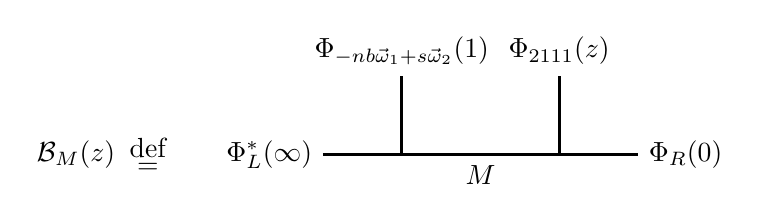
\begin{tikzpicture}
[line width=1.2pt]
\draw (-2.5,0)node[left]{$\cB_M (z)$};
\draw (-2.5,0) node[right]{$\mydef$};
\draw (0,0)--(1,0);
\draw (1,0)--(1,1);
\draw (1,0)--(3,0);
\draw (3,0)--(3,1);
\draw (3,0)--(4,0);
\draw (0,0) node[left]{$\Phi^*_L (\infty)$};
\draw (1,1) node[above]{$\Phi_{- n b \vec{\omega}_1+s\vec{\omega}_2} (1)$};
\draw (3,1) node[above]{$\Phi_{2111} (z)$};
\draw (4,0) node[right]{$\Phi_R (0)$};
\draw (2,0) node[below]{$M$};
\end{tikzpicture}
\end{equation}

The field $\Phi_{- n b \vec{\omega}_1+s\vec{\omega}_2}$ has one null-vector at level $n+1$. In principle one can compute the exact expression of the  corresponding null-vector. This provides the last relation needed to derive the  differential equation satisfied by $\cB_M(z)$. However this is in practice not doable. On the other hand we can argue that the Fuchsian differential equation is associated to a rigid system and therefore can be directly derived by local data.


\section{Differential equations and conformal blocks}

\paragraph{The order of the differential equation.} Let us consider first the $s-$ channel $(z=0)$. From the fusion rules 
$\Phi_{-b \vec{\omega}_1} (z)\Phi_{R}(0)$,  we have three possible fusions
\begin{eqnarray}
\text{Fusion 1:}\quad 
\vec{\alpha}_M^{(s)} &=& \vec{\alpha}_R- b \,     \vec{\omega}_1 \\
\text{Fusion 2:}\; \quad 
      \vec{\alpha}_M^{(s)} &=& \vec{\alpha}_R+ b \, \ll \vec{\omega}_1 - \vec{\omega}_2 \rr   \\
\text{Fusion 3:}\;\quad
\vec{\alpha}_M^{(s)} &=& \vec{\alpha}_R+ b \,     \vec{\omega}_2  
\end{eqnarray}

The above three channels determines the local exponents at $z=0$:
\begin{equation}
\cB_M(z) = z^{\alpha_M}\left(1+a_1 z +a_2 z^2+\cdots..\right),
\end{equation}
where $\alpha_{M} = -\Delta_{R}-\Delta_{-b \vec{\omega}_1}+\Delta_{\vec{\alpha}_M^{(s)}}$. Moreover we predict that the coefficients $a_1, \cdots, a_{n}$ are not fixed,i.e. there is a $n+1-$ dimensional space of solutions having the same local exponent. This can be deduced from the fact that the matrix elements 
\be 
\left< \Phi_{M}(0) W_{-1}^{l}\Phi_{-n b \vec{\omega}_1+s \vec{\omega}_2 }(1) \Phi_{L}(\infty)\right>\;,
\ee 
with $l=1,2,\cdots,n$ cannot be determined. The differential equation is therefore of order $3(n+1)$, and the local exponents  multiplicity at 
 \begin{equation}
 z=0: (n+1,n+1,n+1) \quad z=\infty: (n+1,n+1,n+1)
 \end{equation}
 (the arguments at $z=\infty$ are the same).

At $z=1$ we have the following fusions:
 \begin{eqnarray}
\text{Fusion 1:}\quad 
\vec{\alpha}_{M_1}^{(t)} &=& - b(n+1) \,     \vec{\omega}_1 +s \vec{\omega}_2 \\
\text{Fusion 2:}\; \quad 
      \vec{\alpha}_{M_2}^{(t)} &=& - b(n-1) \,     \vec{\omega}_1 +(s-b) \vec{\omega}_2    \\
\text{Fusion 3:}\;\quad
\vec{\alpha}_{M_{3}}^{(t)} &=& - b n \,     \vec{\omega}_1 +(s+b) \vec{\omega}_2  
\end{eqnarray} 
So one can see that the internal channel is respectively degenerate at level $n+2$, $n$ and $n+1$ respectively. 
Again, using the fact that, if $\Phi_{M}(1)$ is degenerate at level $n+1$, the  $\left< W_{-1}^{l}\Phi_{M}(1) \Phi_{L}(\infty) \Phi_{R}(0)\right>$ are not determined for $l=1,2..n$, we expect that:
 
 \begin{equation}
 z=1: (n+2,n+1,n) 
 \end{equation}
 So the set of multiplicities is expected to be:
 \begin{equation}
 (n+1,n+1,n+1;\; n+2,n+1,n;\; n+1,n+1,n+1)\;,
\end{equation} 
which corresponds to a rigid system. 
For $n=0$ one recovers the result corresponding to the one-level semi-degenerate fields, which corresponds to third order generalized hypergeometric functions. The $n=1$ is the case studied recently by us. 



\paragraph{What is known and what is not.}

The {\it local} $W_N$ four-point {\it correlation functions}:
\begin{equation}
G(z,\bar{z})\mydef\left< \Phi_{R}(0) \Phi_{-b \vec{\omega}_1}(z,\bar{z})\Phi_{- n b \vec{\omega}_1+s \vec{\omega}_2}(1)\Phi_{L}(\infty) \right>
\end{equation}
have been computed in \cite{fl08}, see (Eq 4.12),  and are expressed via {\bf $4 n +4$} dimensional integral. The function $G(z,\bar{z})$ is  a quadratic expression of the conformal block $\cB_M(z)$. For $W_3$, should be related to the conformal blocks (solutions of the differential equations) by:
\begin{equation}
G(z,\bar{z}) = \sum_{i=1}^{3} C(\vec{\alpha}_R, -b\vec{\omega}_1, \vec{\alpha}^{(s)}_{M_i})C(\vec{\alpha}_L, -n b\vec{\omega}_1+s \vec{\omega}_2, \vec{\alpha}^{(s)}_{M_i})\left( \sum_{k,l=1}^{\text{multipl}}a_{k,l}\cB^{(k)}_{M_i}(z)\cB^{(l)}_{M_i}(\bar{z}) \right)
\end{equation}
The structure constants $C$ above have been computed, see (Eq 3.11) of arXiv:0810.3020v2. 


\paragraph{Things to do.}
In our approach it would be interesting:
\begin{itemize}
\item By using the global properties (monodromy group) of our Fuchsian system:
\begin{itemize}
\item check on a more general case that the constraints {\bf imposed by demanding simple monodromy} of the correlation function fixes the structure constants and the $a_{k,l}$. We explicitly carried out this computation in arXiv:1602.03870v2, section 5, for a special case (the diff equation is of fourth order).

\item  {\bf re-derive the above structure constants} and  computing the $a_{k,l}$ once a basis has been chosen 
\end{itemize}

\item Provide integrable expression for $\cB_{M}$. Are they $2 n+2$ integrals or have simpler form?
 
\item The knowledge of the diff equation give access to the three-point functions between descendant fields. These elements are in general not known ( see for instance \cite{Bouwknegt:1992wg} or the collection of works in the book by Schoutens and Bouwknegt-Schoutens) ) and {\bf cannot} be derived by the knowledge of the entire correlation function
\end{itemize}




\section{Third-order differential equation: (111,21,111)}

As a simple example we consider Pochgamer hypergeometric differential equation of rank 3 which in our context arises for
the conformal block with one degenerate field with the parameter $\alpha_1=b\omega_1$ and one 
semi-degenerate with the parameter $\alpha_3= \kappa \omega_2$
\begin{multline}\label{Pochgamer}
  \left[x\left(x\frac{d}{dx}+A_1\right)
  \left(x\frac{d}{dx}+A_2\right)
  \left(x\frac{d}{dx}+A_3\right)-\right.\\-\left.
  \left(x\frac{d}{dx}+B_1-1\right)
  \left(x\frac{d}{dx}+B_2-1\right)x\frac{d}{dx}\right]G(x)=0\;.
\end{multline}
This differential equation of order three has $2+1$ singularities at $0, 1$ and $\infty$. We refer the reader to \cite{yoshida1987fuchsian} for an exhaustive overview of 
Fuchsian systems. In Riemann-symbol notation
the local exponents $\rho^{0}_i,\rho^{1}_i$ and $\rho^{\infty}_i$, $i=1,\cdots,3$, associated to the $2+1$ singular points $0,1$ and $\infty$ can be represented as

\begin{equation}
\label{Riem_not}
\begin{Bmatrix}  
0& & 1 & & \infty  \\ 
0   & &  0   & & A_1   \\
1-B_1  & &  1   & & A_2   \\
1-B_2   & &  -A_1-A_2-A_3+B_1+B_2  & & A_3  
\end{Bmatrix}
\end{equation}

\noindent In terms of the conformal block parameters (see, e.g. \cite{fl07c}, p.17)
\begin{equation}
    A_k=\frac{b\varkappa}{3}-\frac{2}{3}b^2+b(\alpha_1-Q,h_1)+b(\alpha_2-Q,h_k), \quad k=1,2,3
\end{equation}  
and
\begin{equation}
  \begin{aligned}
   B_1=1+b(\alpha_1-Q,e_1)\;, \quad B_2=1+b(\alpha_1-Q,e_1+e_2)\;.
  \end{aligned}
\end{equation}
It is easily checked that \eqref{Pochgamer} is Fuschsian differential equation: the above local exponents satisfy the Fuchs identity:
\begin{equation}
\sum_{i=1}^{n} \left(\rho^0_{i}+\rho^1_{i}+\rho^\infty_{i} \right) = (k-1)\frac{n(n-1)}{2} \;,
\end{equation}
where $n$ is the rank and $k+1$ is the number of singularities. In our case $n=3$ and $k=2$ so that RHS $=3$.
Since the solutions of the differential equation with diagonal monodromies  around $0,1,\infty$  give
correspondingly $s,t,u$ conformal blocks, the  exponents can be found by using $\cW_3$ fusion rules as explained in the previous section. 

In the present case, the set of the multiplicities $m=(\{m_i^{(0)}\}, \{m_j^{(1)}\},\{m_k^{(\infty)}\})$ is
\be\label{multiplic}
m=(111,21,111)=(1^3,21,1^3)=\ll \tableau{1 1 1}, \tableau{2 1}, \tableau{1 1 1}\rr\;.
\ee
Using \eqref{indR} one can verify that the differential equation is rigid
\be
\text{idx}(m)  = - 3^2 + 7 + 4 =2\;,
\ee
Using partitions representation in \eqref{multiplic} we identify $m_{j,\nu}$
with the length of  $\nu$th row in the diagram  $j$. In our convention  $j=0,1,2$  label correspondingly singular points: $(0,1,\infty)$. In this particular case 
\be\label{mults}
m_{1,1}=2\quad \text{and} \quad m_{0,\nu}=m_{2,\nu}=m_{1,2}=1\quad \text{for} \quad \nu=1,2,3\;.
\ee
And the corresponding characteristic exponents are
\begin{align}\label{lambds}
& \lambda_{0,1}=0,\,\lambda_{0,2}=1-B_1,\,\lambda_{0,3}=1-B_2\;,\nonumber\\
& \lambda_{1,1}=0,\, \lambda_{1,2}= -A_1-A_2-A_3+B_1+B_2\;,\\
&  \lambda_{2,1}=A_1,\,\lambda_{2,2}=A_2,\,\lambda_{2,3}=A_3\;.\nonumber
\end{align}


\paragraph{Inverse problem.} Now let us suppose that we know that the differential equation is rigid and we are given by the set of multiplicities \eqref{multiplic}.

It is instructive to introduce the following useful notations 
\be
\text{ord}(m)=\sum_{\nu=1}^\infty m_{j,\nu}\;,
\ee
which does not depend on $j$. Clearly  the order of $m$ it is equal to the rank of our differential equation 
\be 
\text{ord}(m)=n=3\;.
\ee 
Written in terms 
of $\{m_{j,\nu}\}$ the index of rigidity \eqref{indR} reads 
\be\label{indR1}
\text{idx}(m) =(2-p) \text{ord}(m)^2 +\sum_{j=0}^{p-1}\sum_{\nu=0}^\infty m_{j,\nu}^2=2\;.
\ee
We notice that the sets \eqref{mults} and \eqref{lambds} satisfy the following relation
\be
|\{\lambda_m\}|=0\;,
\ee
where
\be
|\{\lambda_m\}|\equiv
\sum_{j=0}^{p-1}\sum_{\nu=1}^{n_j} m_{j,\nu}\lambda_{j,\nu}-\text{ord}(m)+\frac{\text{idx}(m)}{2}\;.
\ee
In general, all information is contained in $p$ tuples of partitions $m_j$, $j=0,...,p-1$, and associated local exponents data $\lambda_m$.

\paragraph{Katz algorithm for constructing rigid tuples.} 
Let us write a Fuchsian differential equation in the linear system form
\be
\frac{\partial Y}{\partial x}=
\bigg(\sum_{j=0}^{p-1} \frac{A_j}{x-x_j}\bigg)Y\;,
\ee
where in our case $p=3$, $x_0=0, x_1=1$ and we also identify $x_{p=2}=\infty$, so that the residue at $x_2$ is $A_2=-A_1-A_2$.

Essentially, the  Katz algorithm consists of two operations:
{\it addition} and {\it middle convolution}.\\
For $\alpha_j\in\mathbb{C}$, $j=0,...,p-1$,  the {\it addition} is defined by
\be
(A_0,\dots, A_{p-1})\mapsto (A_0+\alpha_{0},\dots, A_{p-1}+\alpha_{p-1})\;.
\ee
For $\lambda\in\mathbb{C}$ the {\it convolution} is defined by
\be
(A_0,\dots, A_{p-1})\mapsto (G_0,\dots, G_{p-1})\;,
\ee
where $G_j$ is square matrix $(p-1) n \times (p-1) n$ (n is the rank of the system)
with only one non-zero row
\be
(G_j)_{ik}=\delta_{ij} (A_k+\delta_{kj} \lambda)\;.
\ee

One can prove (see, e.g. \cite{oshima}) that the addition and the middle convolution do not change the index of rigidity.
 
The procedure consist of certain combination of middle convolution operations and addition operations.
The sequence of the operations  can be defined from the sequence  of spectral type changes, leading to the trivial one.
The number and the form of the convolutions is defined  by the parameter
\be 
d=\sum_{j=0}^{p-1} m_1^{(j)}-(p-2)n\;.
\ee
This operation reduces the lengths of the first rows in the diagrams $m^{(j)}$ (defining  spectral type) by $d$ and removes the first row if it becomes zero.\footnote{In case if it becomes negative the corresponding spectral type is not irreducibly realizable.}

In our example the sequence of spectral types is obtained in two steps which reduce partitions 
\be (111,21,111)\xrightarrow{d}(011,11,011)=(11,11,11)\xrightarrow{d'}(01,01,01)=(1,1,1)
\ee
and the corresponding values $d=1$ and $d'=1$. Hence in order to come from rank 1 to rank 3 system
(i.e. to go in the opposite direction) we have to apply middle convolution twice.

Notice that the middle convolution is additive, which means
\be
mc_a mc_b = mc_{a+b}\;.
\ee
So that the iteration of two middle convolutions gives the same result of one middle convolution.

So in order to obtain a system of spectral type (111,21,111),
we first operate middle convolution to (1,1,1) equation, and get a system of spectral type (11,11,11).
Next, we want to change the first spectral type 11 to 111 
and the second spectral type11 to 21 by a middle convolution.
For this purpose, before middle convolution,
we operate an addition to the first residue matrix so that it does not have the kernel.
Then we will get (111,21,111) system by a middle convolution of arbitrary parameter. 


\section{Fourth-order differential equation: (???)}
Here we apply described methods for Katz system in the case considered in \cite{Belavin:2016qaa}.

\section{Sixth-order differential equation: (222,321,222)}
Here we apply described methods for Katz system in the case considered in \cite{Belavin:2016wlo}.
The  correlation $G(z,\bar{z})$  
\be
G(z,\bar{z})=\langle V_{-b \omega_1}(z,\bar{z}) V_{\alpha_1}(0) V_{\alpha_2}(1)V_{\kappa \omega_2-b \omega_1}(\infty)\rangle\;.
\ee
in $\cW_3$ Toda CFT.

\subsection{Integral representation of solutions}
In \cite{fl08} the following integral representation for the correlation function\footnote{In fact,  the proposed expression is for more general case with the last field $V_{\kappa \omega_2-n b \omega_1}$.} has been proposed
\begin{align}
G(z,\bar{z})=&|z|^{2b (\alpha_1,\omega_1)}|z-1|^{2b (\alpha_2,\omega_1)}\int\int\int\int\, d^2 t_1d^2 t_2d^2 y_1d^2 y_2\,\,
|t_1-z|^{2\delta}\times\nonumber\\
& 
 |t_1|^{2\alpha}|t_1-1|^{2\beta} |t_1-y_1|^{2\gamma}\times\nonumber\\
&|y_1|^{2\alpha'}|y_1-1|^{2\beta'}|y_1-t_2|^{-2b^2}\times\nonumber\\
&|t_2|^{-2(1+\alpha)}|t_2-1|^{-2(1+\beta)}|t_2-y_2|^{-2(1+\gamma)}\times\nonumber\\
&|y_2|^{-2(1+\alpha')}|y_2-1|^{-2(1+\beta')}\;,
\end{align}
where parameters are... 


\section{Ninth-order differential equation: (333,432,333)}

\section{From monodromy to structure constants}

\subsection{Invariant Hermitian form}

It may be interesting to calculate the invariant Hermitian form for the monodromy group.
I think that the invariant Hermitian form can be also obtained in a recursive way by the Katz algorithm.
For the invariant Hermitian form, the following references are useful: \\\\
Y. Haraoka, Monodromy representations of systems of differential equations free from accessory parameters,
SIAM J. Math. Anal., 25 (1994), 1595-1621.\\\\
The invariant Hermitian form for a differential equation having integral representation of solutions of Euler type
can also be obtained by the intersection form of twisted cycles.
The reference is:\\\\
M. Kita and M. Yoshida, Intersection theory for twisted cycles,
Math. Nachr., 166 (1994), 287-304.

\section{Summary and discussion}
\label{summary}


The presented consideration can be useful to clarify  general classification of Fuchsian equations appearing in the context of the conformal field theories with different types of chiral algebras.  We believe  that entering  this problem we can get to more general features of CFTs. Another interesting point is that in general case indices of CFT-like Fucks equations and in particular of the BPZ equation \cite{bpz84} are not equal to 2 and hence are not rigid. So there are CFT conformal blocks not necessarily representing subject of rigid Fucksian systems. It is interesting to clarify the conditions of rigidity  of CFT-Fucks equations and whether or not similar methods are applicable in non-rigid cases. 


\appendix






\bibliographystyle{JHEP}
\bibliography{bibnonwy.bib}


\end{document}
